% Options for packages loaded elsewhere
\PassOptionsToPackage{unicode}{hyperref}
\PassOptionsToPackage{hyphens}{url}
\PassOptionsToPackage{dvipsnames,svgnames,x11names}{xcolor}
%
\documentclass[
]{article}
\usepackage{amsmath,amssymb}
\usepackage{lmodern}
\usepackage{setspace}
\usepackage{iftex}
\ifPDFTeX
  \usepackage[T1]{fontenc}
  \usepackage[utf8]{inputenc}
  \usepackage{textcomp} % provide euro and other symbols
\else % if luatex or xetex
  \usepackage{unicode-math}
  \defaultfontfeatures{Scale=MatchLowercase}
  \defaultfontfeatures[\rmfamily]{Ligatures=TeX,Scale=1}
\fi
% Use upquote if available, for straight quotes in verbatim environments
\IfFileExists{upquote.sty}{\usepackage{upquote}}{}
\IfFileExists{microtype.sty}{% use microtype if available
  \usepackage[]{microtype}
  \UseMicrotypeSet[protrusion]{basicmath} % disable protrusion for tt fonts
}{}
\makeatletter
\@ifundefined{KOMAClassName}{% if non-KOMA class
  \IfFileExists{parskip.sty}{%
    \usepackage{parskip}
  }{% else
    \setlength{\parindent}{0pt}
    \setlength{\parskip}{6pt plus 2pt minus 1pt}}
}{% if KOMA class
  \KOMAoptions{parskip=half}}
\makeatother
\usepackage{xcolor}
\IfFileExists{xurl.sty}{\usepackage{xurl}}{} % add URL line breaks if available
\IfFileExists{bookmark.sty}{\usepackage{bookmark}}{\usepackage{hyperref}}
\hypersetup{
  pdftitle={A general model for the evolution of nuptial gift-giving: Supporting Information},
  colorlinks=true,
  linkcolor={blue},
  filecolor={Maroon},
  citecolor={Blue},
  urlcolor={Blue},
  pdfcreator={LaTeX via pandoc}}
\urlstyle{same} % disable monospaced font for URLs
\usepackage[margin=1in]{geometry}
\usepackage{color}
\usepackage{fancyvrb}
\newcommand{\VerbBar}{|}
\newcommand{\VERB}{\Verb[commandchars=\\\{\}]}
\DefineVerbatimEnvironment{Highlighting}{Verbatim}{commandchars=\\\{\}}
% Add ',fontsize=\small' for more characters per line
\usepackage{framed}
\definecolor{shadecolor}{RGB}{248,248,248}
\newenvironment{Shaded}{\begin{snugshade}}{\end{snugshade}}
\newcommand{\AlertTok}[1]{\textcolor[rgb]{0.94,0.16,0.16}{#1}}
\newcommand{\AnnotationTok}[1]{\textcolor[rgb]{0.56,0.35,0.01}{\textbf{\textit{#1}}}}
\newcommand{\AttributeTok}[1]{\textcolor[rgb]{0.77,0.63,0.00}{#1}}
\newcommand{\BaseNTok}[1]{\textcolor[rgb]{0.00,0.00,0.81}{#1}}
\newcommand{\BuiltInTok}[1]{#1}
\newcommand{\CharTok}[1]{\textcolor[rgb]{0.31,0.60,0.02}{#1}}
\newcommand{\CommentTok}[1]{\textcolor[rgb]{0.56,0.35,0.01}{\textit{#1}}}
\newcommand{\CommentVarTok}[1]{\textcolor[rgb]{0.56,0.35,0.01}{\textbf{\textit{#1}}}}
\newcommand{\ConstantTok}[1]{\textcolor[rgb]{0.00,0.00,0.00}{#1}}
\newcommand{\ControlFlowTok}[1]{\textcolor[rgb]{0.13,0.29,0.53}{\textbf{#1}}}
\newcommand{\DataTypeTok}[1]{\textcolor[rgb]{0.13,0.29,0.53}{#1}}
\newcommand{\DecValTok}[1]{\textcolor[rgb]{0.00,0.00,0.81}{#1}}
\newcommand{\DocumentationTok}[1]{\textcolor[rgb]{0.56,0.35,0.01}{\textbf{\textit{#1}}}}
\newcommand{\ErrorTok}[1]{\textcolor[rgb]{0.64,0.00,0.00}{\textbf{#1}}}
\newcommand{\ExtensionTok}[1]{#1}
\newcommand{\FloatTok}[1]{\textcolor[rgb]{0.00,0.00,0.81}{#1}}
\newcommand{\FunctionTok}[1]{\textcolor[rgb]{0.00,0.00,0.00}{#1}}
\newcommand{\ImportTok}[1]{#1}
\newcommand{\InformationTok}[1]{\textcolor[rgb]{0.56,0.35,0.01}{\textbf{\textit{#1}}}}
\newcommand{\KeywordTok}[1]{\textcolor[rgb]{0.13,0.29,0.53}{\textbf{#1}}}
\newcommand{\NormalTok}[1]{#1}
\newcommand{\OperatorTok}[1]{\textcolor[rgb]{0.81,0.36,0.00}{\textbf{#1}}}
\newcommand{\OtherTok}[1]{\textcolor[rgb]{0.56,0.35,0.01}{#1}}
\newcommand{\PreprocessorTok}[1]{\textcolor[rgb]{0.56,0.35,0.01}{\textit{#1}}}
\newcommand{\RegionMarkerTok}[1]{#1}
\newcommand{\SpecialCharTok}[1]{\textcolor[rgb]{0.00,0.00,0.00}{#1}}
\newcommand{\SpecialStringTok}[1]{\textcolor[rgb]{0.31,0.60,0.02}{#1}}
\newcommand{\StringTok}[1]{\textcolor[rgb]{0.31,0.60,0.02}{#1}}
\newcommand{\VariableTok}[1]{\textcolor[rgb]{0.00,0.00,0.00}{#1}}
\newcommand{\VerbatimStringTok}[1]{\textcolor[rgb]{0.31,0.60,0.02}{#1}}
\newcommand{\WarningTok}[1]{\textcolor[rgb]{0.56,0.35,0.01}{\textbf{\textit{#1}}}}
\usepackage{longtable,booktabs,array}
\usepackage{calc} % for calculating minipage widths
% Correct order of tables after \paragraph or \subparagraph
\usepackage{etoolbox}
\makeatletter
\patchcmd\longtable{\par}{\if@noskipsec\mbox{}\fi\par}{}{}
\makeatother
% Allow footnotes in longtable head/foot
\IfFileExists{footnotehyper.sty}{\usepackage{footnotehyper}}{\usepackage{footnote}}
\makesavenoteenv{longtable}
\usepackage{graphicx}
\makeatletter
\def\maxwidth{\ifdim\Gin@nat@width>\linewidth\linewidth\else\Gin@nat@width\fi}
\def\maxheight{\ifdim\Gin@nat@height>\textheight\textheight\else\Gin@nat@height\fi}
\makeatother
% Scale images if necessary, so that they will not overflow the page
% margins by default, and it is still possible to overwrite the defaults
% using explicit options in \includegraphics[width, height, ...]{}
\setkeys{Gin}{width=\maxwidth,height=\maxheight,keepaspectratio}
% Set default figure placement to htbp
\makeatletter
\def\fps@figure{htbp}
\makeatother
\setlength{\emergencystretch}{3em} % prevent overfull lines
\providecommand{\tightlist}{%
  \setlength{\itemsep}{0pt}\setlength{\parskip}{0pt}}
\setcounter{secnumdepth}{-\maxdimen} % remove section numbering
\newlength{\cslhangindent}
\setlength{\cslhangindent}{1.5em}
\newlength{\csllabelwidth}
\setlength{\csllabelwidth}{3em}
\newlength{\cslentryspacingunit} % times entry-spacing
\setlength{\cslentryspacingunit}{\parskip}
\newenvironment{CSLReferences}[2] % #1 hanging-ident, #2 entry spacing
 {% don't indent paragraphs
  \setlength{\parindent}{0pt}
  % turn on hanging indent if param 1 is 1
  \ifodd #1
  \let\oldpar\par
  \def\par{\hangindent=\cslhangindent\oldpar}
  \fi
  % set entry spacing
  \setlength{\parskip}{#2\cslentryspacingunit}
 }%
 {}
\usepackage{calc}
\newcommand{\CSLBlock}[1]{#1\hfill\break}
\newcommand{\CSLLeftMargin}[1]{\parbox[t]{\csllabelwidth}{#1}}
\newcommand{\CSLRightInline}[1]{\parbox[t]{\linewidth - \csllabelwidth}{#1}\break}
\newcommand{\CSLIndent}[1]{\hspace{\cslhangindent}#1}
\usepackage{amsmath}
\usepackage{natbib}
\usepackage{lineno}
\usepackage{caption}
\usepackage[utf8]{inputenc}
\bibliographystyle{amnatnat}
\ifLuaTeX
  \usepackage{selnolig}  % disable illegal ligatures
\fi

\title{A general model for the evolution of nuptial gift-giving:
Supporting Information}
\author{Author list (anonymised)}
\date{{[}1{]} Author institutions and email}

\begin{document}
\maketitle

\setstretch{1}
\hypertarget{table-of-contents}{%
\section{Table of Contents}\label{table-of-contents}}

\begin{longtable}[]{@{}ll@{}}
\toprule
Information & Page \\
\midrule
\endhead
S1: Alternative derivation of male fitness threshold & 2 \\
S2: Operational sex ratio & 4 \\
S3: Sensitivity analysis of parameters in IBM & 5 \\
S4: Separate evolution of male search and female choice & 12 \\
References & 13 \\
\bottomrule
\end{longtable}

\clearpage

\hypertarget{s1-alternative-derivation-of-male-fitness-threshold}{%
\subsection{S1: Alternative derivation of male fitness
threshold}\label{s1-alternative-derivation-of-male-fitness-threshold}}

In the main text, we assumed that males made the decision to search or
not search for a nuptial gift. The expected length of time for which
searching males are expected to remain outside of the mating pool is
\(E[T_{\mathrm{m}}] = \alpha\) (see Model). Alternatively, we can assume
that males search for a period of \(T_{\mathrm{m}}\) and spend this full
duration of \(T_{\mathrm{m}}\) in the time-out phase, even if they
succeed in finding a nuptial gift (as we assumed in our IBM). The
probability that a male obtains a nuptial gift during this time is
modelled in Eq. 1,

\[P(G) = 1 - e^{-\frac{1}{\alpha}T_{\mathrm{m}}}.\]

In Eq. 1, \(\alpha\) is the amount of time expected to pass before a
male encounters a nuptial gift. We assume that a male will only enter
the mating pool with no gift if they are unsuccessful in obtaining a
gift, so the probability that a male obtains no gift after
\(T_{\mathrm{m}}\) is,

\[P(L) = e^{-\frac{1}{\alpha}T_{\mathrm{m}}}.\]

We assume that the fitness increment in reproductive success associated
with receiving a nuptial gift versus no nuptial gift are
\(\lambda(1 + \gamma)\) and \(\lambda\), respectively. The rate at which
males increase their fitness can then be defined as the expected fitness
increment from their nuptial gift search divided by \(T_{\mathrm{m}}\)
plus the time spent in the mating pool waiting to encounter a mate,

\[W_{\mathrm{m}} = \lambda \frac{P(G)\left(1 + \gamma\right) + P(L)}{T_{\mathrm{m}} + \left( \frac{\beta + 1}{R} \right)}.\]

Our objective now is to determine the conditions under which a focal
male increases his fitness by searching for a nuptial gift
(\(T_{\mathrm{m}}>0\)) in a population of resident males that do not
search (\(T_{\mathrm{m}}=0\)). Females are assumed to exhibit no
choosiness for males with versus without nuptial gifts. Under such
conditions, male fitness cannot be affected by female choice, so
selection to increase \(T_{\mathrm{m}}>0\) must be based solely on
\(\alpha\), \(\beta\), \(R\), and \(\gamma\).

To determine under what conditions male inclusive fitness increases with
nuptial gift search time, we can differentiate \(W_{\mathrm{m}}\) with
respect to \(T_{\mathrm{m}}\),

\[\frac{\partial W_{\mathrm{m}}}{\partial T_{\mathrm{m}}} = \lambda\frac{\gamma\left(\frac{\frac{T_{\mathrm{m}} + \frac{\beta + 1}{R}}{\alpha} + 1}{e^{\frac{1}{\alpha}T_{\mathrm{m}}}} - 1\right) - 1}{\left(T_{\mathrm{m}} + \frac{\beta + 1}{R} \right)^{2}}.\]

Because \(T_{\mathrm{m}} = 0\), the above simplifies,

\[\frac{\partial W_{\mathrm{m}}}{\partial T_{\mathrm{m}}} = \lambda \frac{\frac{R\gamma\left(\beta + 1\right)}{\alpha} - R^{2}}{\left(1 + \beta \right)^{2}}.\]

We can re-arrange the above,

\[\frac{\partial W_{\mathrm{m}}}{\partial T_{\mathrm{m}}} = \lambda \frac{R\gamma}{\alpha\left(\beta+1\right)} - \lambda\frac{R^{2}}{{\left(1 + \beta \right)^{2}}}.\]

Note that if \(R = 0\) or \(\lambda = 0\), then, trivially, no change in
fitness occurs (since females and males cannot mate or do not produce
offspring). Fitness is increased by searching for nuptial gifts when
\(\gamma\) is high, scaled by the expect search time needed to find a
nuptial gift. A second term on the right-hand side is subtracted, which
reflects a loss in fitness proportional to the encounter rate of
potential mates in the mating pool. The conditions under which male
inclusive fitness increases by searching for a nuptial gift are found by
setting \(\partial W_{\mathrm{m}}/\partial T_{\mathrm{m}} = 0\) and
solving for \(\gamma\) to recover Eq. 2 from the main text,

\[0 = \lambda \frac{R\gamma}{\alpha\left(\beta+1\right)} - \lambda\frac{R^{2}}{{\left(1 + \beta \right)^{2}}},\]

\[\lambda\frac{R^{2}}{{\left(1 + \beta \right)^{2}}} = \lambda \frac{R\gamma}{\alpha\left(\beta+1\right)},\]

\[\frac{R}{{\left(1 + \beta \right)^{2}}} =  \frac{\gamma}{\alpha\left(\beta+1\right)},\]

\[\frac{R}{{\left(1 + \beta \right)}} =  \frac{\gamma}{\alpha},\]

\[\gamma = \alpha \frac{R }{\beta + 1}.\]

\clearpage

\hypertarget{s2-operational-sex-ratio}{%
\subsection{S2: Operational sex ratio}\label{s2-operational-sex-ratio}}

We assume that the ratio of males to females is the same upon individual
maturation. Consequently, the operational sex ratio \(\beta\) will be a
function of \(R\), \(T_{\mathrm{f}}\), and \(T_{\mathrm{m}}\) because
these parameters determine the density of females and males in the
mating pool versus outside of the mating pool. We start with the
definition of \(\beta\) as being the probability of finding an
individual in time-in (\protect\hyperlink{ref-Kokko2001}{Kokko \&
Monaghan, 2001}),

\[\beta = \frac{\int_{t=0}^{\infty}P_{IM}(t)dt}{\int_{t=0}^{\infty}P_{IF}(t)dt}\]

We can substitute the equations for \(P_{IM}(t)\) and \(P_{IF}(t)\),
which define the probabilities of males and females being within the
mating pool at time \(t\), respectively.

We can therefore calculate \(\beta\) as below,

\[\beta = \frac{\left( \frac{\left(\frac{\beta + 1}{R}\right)}{T_{\mathrm{m}} + \left(\frac{\beta + 1}{R}\right)} \right)}{\left( \frac{\left(R \frac{\beta}{\beta + 1}\right)}{T_{\mathrm{f}} + \left(R \frac{\beta}{\beta + 1}\right)} \right)}.\]

This can be simplified,

\[\beta = \frac{\left(\beta\left(R + T_{f}\right) + T_{f}\right)\left(\beta + 1\right)}{\beta \left(R^{2}T_{m} + R\right) + \beta^{2}R}.\]

There is no closed form solution for \(\beta\), but a recursive
algorithm can be used to calculate \(\beta\) to an arbitrary degree of
precision.

\begin{Shaded}
\begin{Highlighting}[]
\NormalTok{recursive\_b }\OtherTok{\textless{}{-}} \ControlFlowTok{function}\NormalTok{(B, D, Tf, Tm, }\AttributeTok{crit =} \FloatTok{0.0001}\NormalTok{, }\AttributeTok{maxit =} \DecValTok{9999}\NormalTok{)\{}
\NormalTok{  conv }\OtherTok{\textless{}{-}} \DecValTok{1}\NormalTok{;}
\NormalTok{  iter }\OtherTok{\textless{}{-}} \DecValTok{0}\NormalTok{;}
  \ControlFlowTok{while}\NormalTok{(conv }\SpecialCharTok{\textgreater{}}\NormalTok{ crit }\SpecialCharTok{\&}\NormalTok{ iter }\SpecialCharTok{\textless{}}\NormalTok{ maxit)\{}
\NormalTok{    Fe   }\OtherTok{\textless{}{-}}\NormalTok{ D }\SpecialCharTok{*}\NormalTok{ (B }\SpecialCharTok{/}\NormalTok{ (}\DecValTok{1} \SpecialCharTok{+}\NormalTok{ B));}
\NormalTok{    Me   }\OtherTok{\textless{}{-}}\NormalTok{ (}\DecValTok{1} \SpecialCharTok{+}\NormalTok{ B) }\SpecialCharTok{/}\NormalTok{ D;}
\NormalTok{    Bn   }\OtherTok{\textless{}{-}}\NormalTok{ (Me }\SpecialCharTok{/}\NormalTok{ (Tm }\SpecialCharTok{+}\NormalTok{ Me)) }\SpecialCharTok{/}\NormalTok{ (Fe }\SpecialCharTok{/}\NormalTok{ (Tf }\SpecialCharTok{+}\NormalTok{ Fe));}
\NormalTok{    iter }\OtherTok{\textless{}{-}}\NormalTok{ iter }\SpecialCharTok{+} \DecValTok{1}\NormalTok{;}
\NormalTok{    conv }\OtherTok{\textless{}{-}} \FunctionTok{abs}\NormalTok{(Bn }\SpecialCharTok{{-}}\NormalTok{ B);}
\NormalTok{    B    }\OtherTok{\textless{}{-}}\NormalTok{ Bn;}
\NormalTok{  \}}
  \FunctionTok{return}\NormalTok{(}\FunctionTok{list}\NormalTok{(}\AttributeTok{B =}\NormalTok{ B, }\AttributeTok{conv =}\NormalTok{ conv, }\AttributeTok{iter =}\NormalTok{ iter));}
\NormalTok{\}}
\end{Highlighting}
\end{Shaded}

We used the above function to calculate values of \(\beta\) for the
analytical model.

\clearpage

\hypertarget{s3-sensitivity-analysis-of-parameters-in-ibm}{%
\subsection{S3: Sensitivity analysis of parameters in
IBM}\label{s3-sensitivity-analysis-of-parameters-in-ibm}}

We investigated the sensitivity of our results to individual mortality
during time-in (\(\mu_{\mathrm{in}}\)) and time-out
(\(\mu_{\mathrm{out}}\)), female processing time (\(T_{\mathrm{f}}\)),
and the potential for interactions between conspecifics (\(\psi\)).
Across all of these simulations, there were challenges with statistical
power. Evidence for the evolution of male search (blue points in
figures) and female choosiness (red points in figures) was determined by
the lower 95\% bootstrapped confidence interval of \(T_{\mathrm{m}}\)
and \(T_{\mathrm{f}}\) values being greater than zero, respectively.
This required a lot of replicate simulations in the main text (Figure
3), especially for values just above predicted thresholds and for female
choosiness. Computation time was a limiting factor, even using a
compiled language (C) and with access to a computing cluster. Absence of
points above threshold values are not necessarily evidence that
evolution of male search or female choosiness is not predicted to evolve
in these regions of parameter space, but it does indicate that evolution
of these traits is not necessarily assured given the stochasticity
inherent to the IBM. Additional simulations can be conducted using the C
code in the `src' folder of the GitHub repository
(\url{https://github.com/AUTHOR_NAME/REPOSITORY_NAME}). Below, we
explain the parameter values used in the sensitivity analysis in more
detail.

\emph{Mortality}

We conducted a sensitivity analysis of the effect of the mortality
parameters \(\mu_{\mathrm{in}}\) and \(\mu_{\mathrm{out}}\) (the
probability of mortality in time-in and time-out, respectively, which we
assumed to be equal for all individuals) on the evolution of male search
and female choice using the IBM. The results revealed no correlation
between the value of the mortality parameters and the evolution of male
search or female choice (Fig. S2.1).

\emph{Female processing time}

We also conducted a sensitivity analysis of female processing time
\(T_{\mathrm{f}}\). To do this, we ran simulations at default values,
but with \(T_{\mathrm{f}} = 10.0\) (Figures S2.2).

\emph{Interactions between conspecifics}

We conducted a sensitivity analysis on the encounter rate between
conspecifics (\(R\)) by varying the value of our scaling parameter
\(\psi\). Under default simulations, \(\psi = 3\). We also ran
simulations in which \(\psi = 1\) (Figure S2.3), \(\psi = 2\) (Figure
S3.4), \(\psi = 4\) (Figure S3.5), and \(\psi = 6\) (Figure S3.6), with
all other parameters being set to default values.

\clearpage

\captionsetup{labelformat=empty}

\begin{figure}
\centering
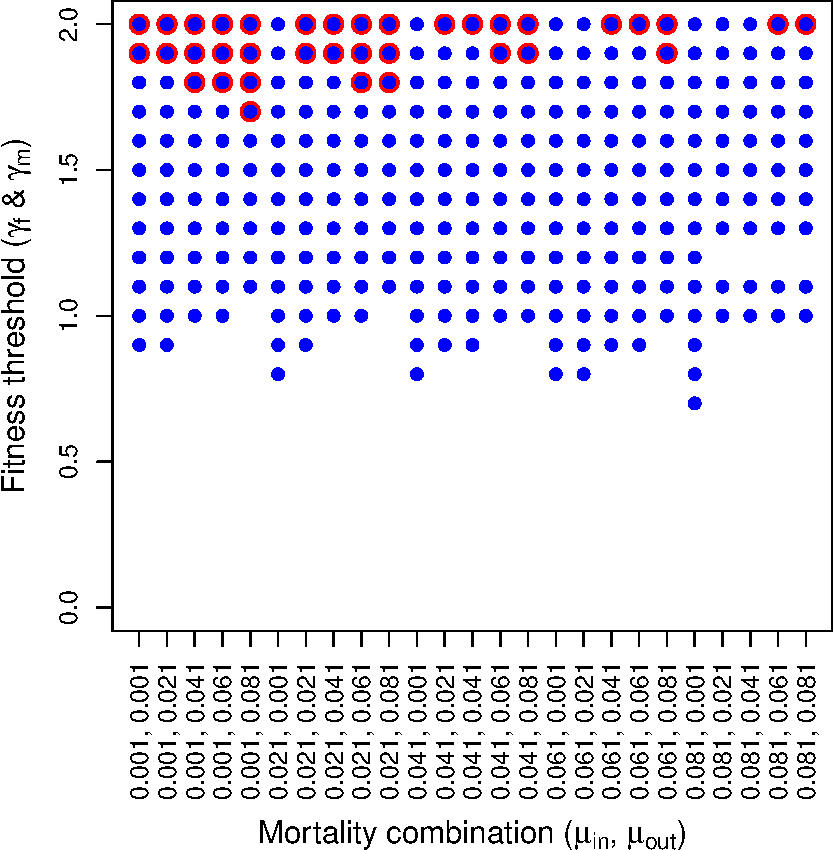
\includegraphics{SI_files/figure-latex/unnamed-chunk-3-1.pdf}
\caption{Figure S2.1: Evolution of both male search (blue) and female
choice (red) under different combinations of the mortality rates
\(\mu_{\mathrm{in}}\) and \(\mu_{\mathrm{out}}\) (mortality in time-in
and out, respectively). The y-axis is the threshold fitness that leads
to evolution of male search (blue) or female choice (red). The results
show noise, but no correlation between the value of the mortality
parameters and the propensity for male search and/or female choice to
evolve. For each of the \(25 \times 20\) combinations of
\(\mu_{\mathrm{in}}\) and \(\mu_{\mathrm{out}}\), 3000 replicate
simulations were run.}
\end{figure}

\captionsetup{labelformat=default}

\clearpage

\captionsetup{labelformat=empty}

\begin{figure}
\centering
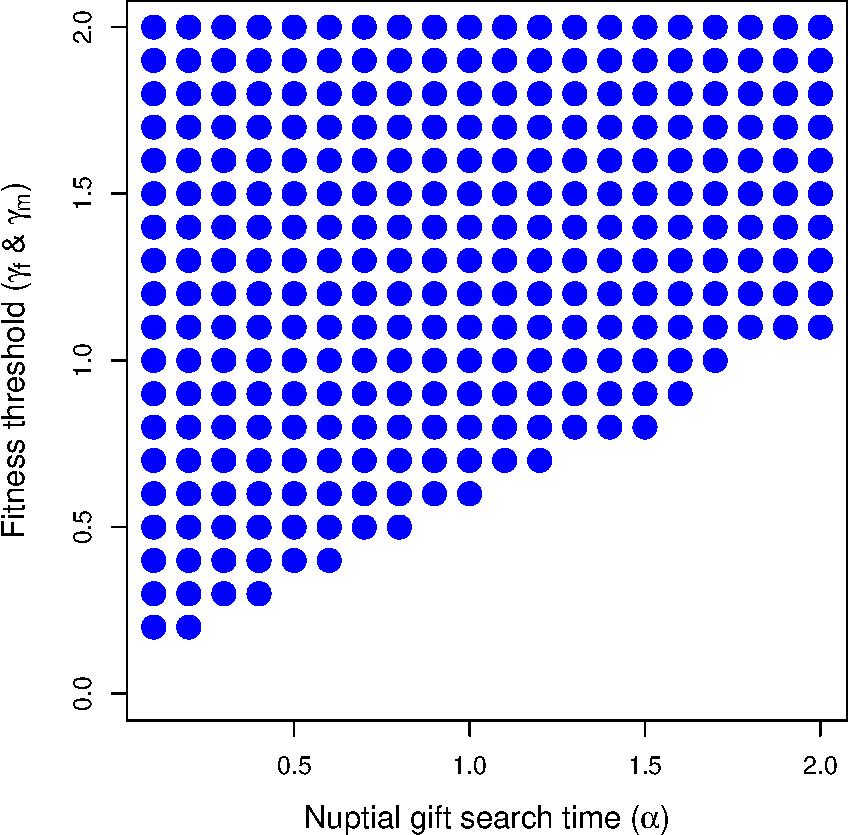
\includegraphics{SI_files/figure-latex/unnamed-chunk-4-1.pdf}
\caption{Figure S2.3 (\(T_{\mathrm{f}} = 10.0\)): The coevolution of
male search and female choosiness as a function of nuptial gift search
time (\(\alpha\)). Points show where the lower 95\% confidence interval
of female choosiness (red) and male search (blue) exceeds zero,
indicating evolution of choosiness or nuptial gift search. Each point
includes data from 3000 replicate simulations with identical starting
conditions. Up to 3000 interactions occur between individuals in each
time step (\(\psi = 3\)), potentially resulting in a mating interaction.
The number of individuals in the population remained at or near carrying
capacity of \(K = 1000\). Expected female processing time was set to
\(T_{\mathrm{f}}=10.0\) time steps, and \(\gamma\) and \(\alpha\) values
in the range {[}0.1, 2.0{]} and {[}0.0, 2.0{]}, respectively, were
used.}
\end{figure}

\captionsetup{labelformat=default}

\clearpage

\captionsetup{labelformat=empty}

\begin{figure}
\centering
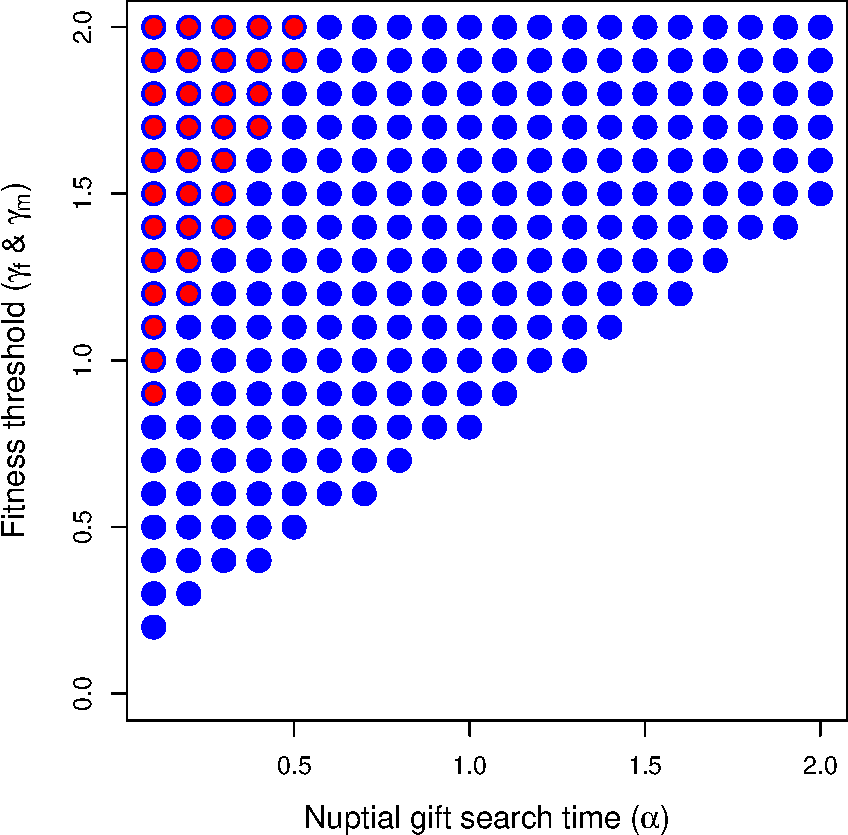
\includegraphics{SI_files/figure-latex/unnamed-chunk-5-1.pdf}
\caption{Figure S2.4 (\(\psi = 1\)): The coevolution of male search and
female choosiness as a function of nuptial gift search time
(\(\alpha\)). Points show where the lower 95\% confidence interval of
where male search (blue) exceeds zero, indicating evolution of
choosiness or nuptial gift search. Each point includes data from 3000
replicate simulations with identical starting conditions. Up to 1000
interactions occur between individuals in each time step (\(\psi = 1\)),
potentially resulting in a mating interaction. The number of individuals
in the population remained at or near carrying capacity of \(K = 1000\).
Expected female processing time was set to \(T_{\mathrm{f}}=2\) time
steps, and \(\gamma\) and \(\alpha\) values in the range {[}0.0, 2.0{]}
and {[}0.1, 2.0{]}, respectively, were used.}
\end{figure}

\captionsetup{labelformat=default}

\clearpage

\captionsetup{labelformat=empty}

\begin{figure}
\centering
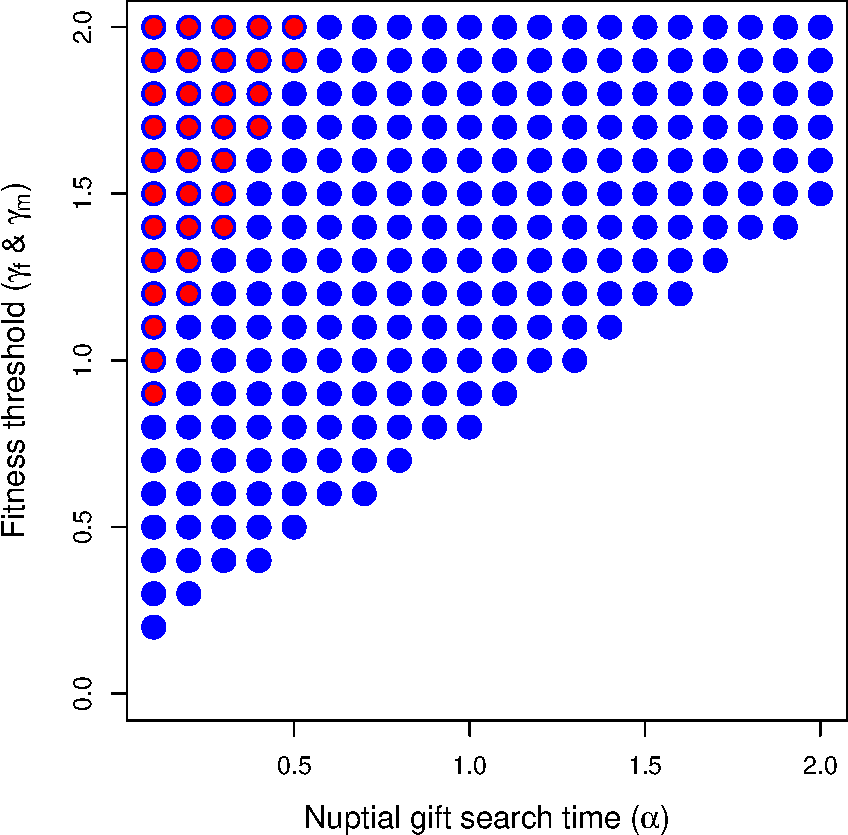
\includegraphics{SI_files/figure-latex/unnamed-chunk-6-1.pdf}
\caption{Figure S2.5 (\(\psi = 2\)): The coevolution of male search and
female choosiness as a function of nuptial gift search time
(\(\alpha\)). Points show where the lower 95\% confidence interval of
where male search (blue) exceeds zero, indicating evolution of
choosiness or nuptial gift search. Each point includes data from 3000
replicate simulations with identical starting conditions. Up to 2000
interactions occur between individuals in each time step (\(\psi = 2\)),
potentially resulting in a mating interaction. The number of individuals
in the population remained at or near carrying capacity of \(K = 1000\).
Expected female processing time was set to \(T_{\mathrm{f}}=2\) time
steps, and \(\gamma\) and \(\alpha\) values in the range {[}0.0, 2.0{]}
and {[}0.1, 2.0{]}, respectively, were used.}
\end{figure}

\captionsetup{labelformat=default}

\clearpage

\captionsetup{labelformat=empty}

\begin{figure}
\centering
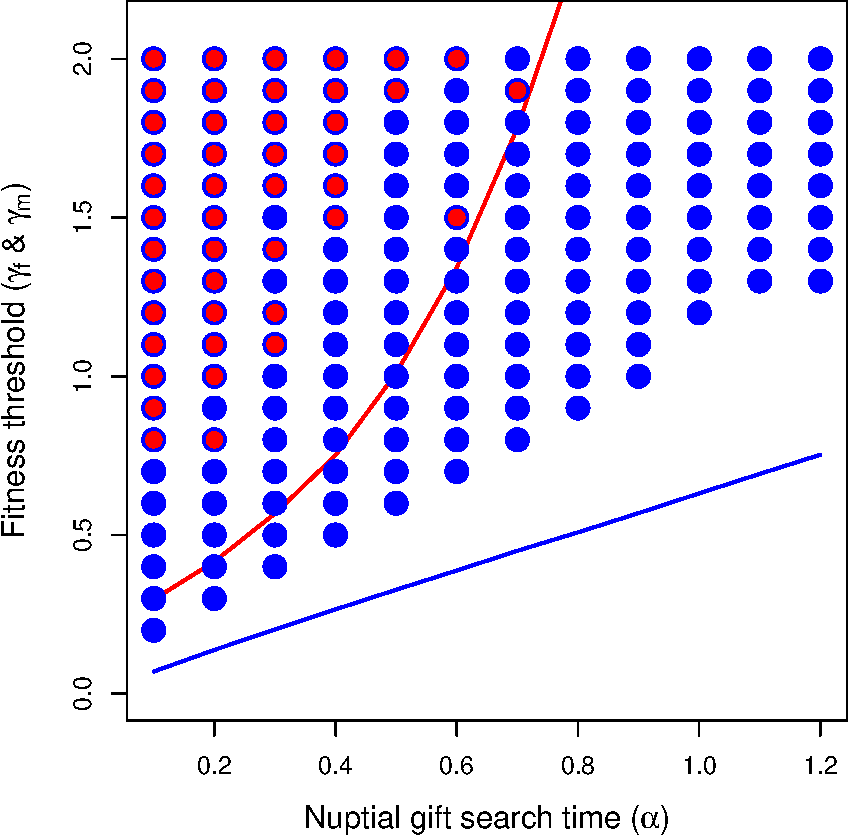
\includegraphics{SI_files/figure-latex/unnamed-chunk-7-1.pdf}
\caption{Figure S2.6 (\(\psi = 4\)): The coevolution of male search and
female choosiness as a function of nuptial gift search time
(\(\alpha\)). Points show where the lower 95\% confidence interval of
where male search (blue) exceeds zero, indicating evolution of
choosiness or nuptial gift search. Each point includes data from 3000
replicate simulations with identical starting conditions. Up to 4000
interactions occur between individuals in each time step, potentially
resulting in a mating interaction (\(\psi = 4\)). The number of
individuals in the population remained at or near carrying capacity of
\(K = 1000\). Expected female processing time was set to
\(T_{\mathrm{f}}=2\) time steps, and \(\gamma\) and \(\alpha\) values in
the range {[}0.0, 2.0{]} and {[}0.1, 2.0{]}, respectively, were used.}
\end{figure}

\captionsetup{labelformat=default}

\clearpage

\captionsetup{labelformat=empty}

\begin{figure}
\centering
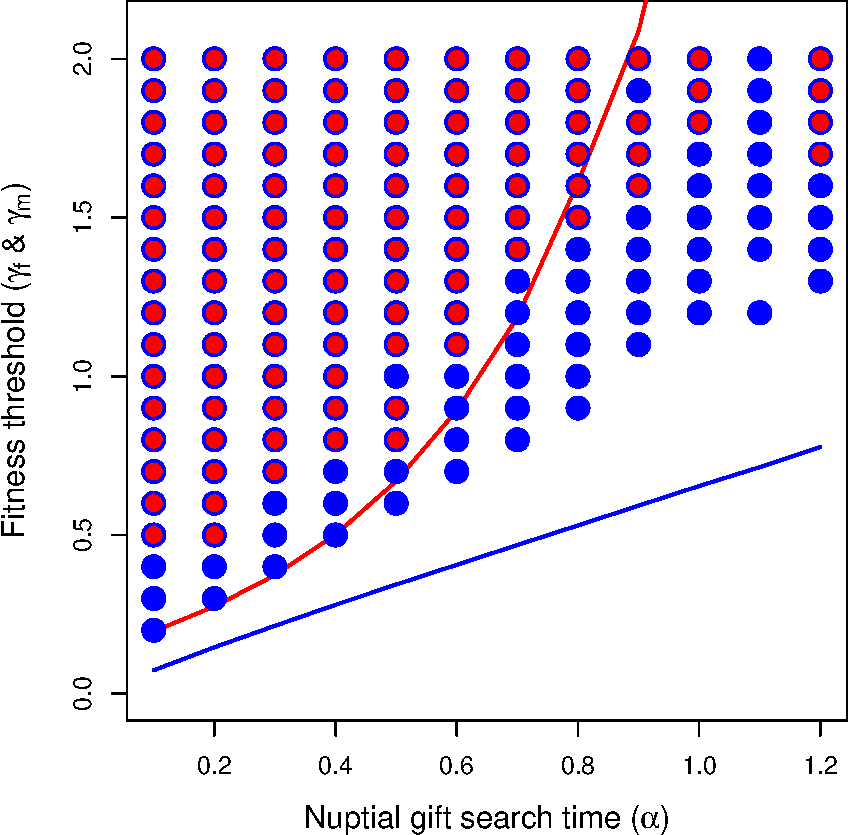
\includegraphics{SI_files/figure-latex/unnamed-chunk-8-1.pdf}
\caption{Figure S2.7 (\(\psi = 6\)): The coevolution of male search and
female choosiness as a function of nuptial gift search time
(\(\alpha\)). Points show where the lower 95\% confidence interval of
where male search (blue) exceeds zero, indicating evolution of
choosiness or nuptial gift search. Each point includes data from 3000
replicate simulations with identical starting conditions. Up to 6000
interactions occur between individuals in each time step, potentially
resulting in a mating interaction (\(\psi = 6\)). The number of
individuals in the population remained at or near carrying capacity of
\(K = 1000\). Expected female processing time was set to
\(T_{\mathrm{f}}=2\) time steps, and \(\gamma\) and \(\alpha\) values in
the range {[}0.0, 2.0{]} and {[}0.1, 2.0{]}, respectively, were used.}
\end{figure}

\captionsetup{labelformat=default}

\clearpage

\hypertarget{s4-separate-evolution-of-male-search-and-female-choice}{%
\subsection{S4: Separate evolution of male search and female
choice}\label{s4-separate-evolution-of-male-search-and-female-choice}}

We used the individual-based simulation model to unpack the effect of
coevolution on the evolution of male search and female choice. Here we
replicated the simulations shown in the main text under the condition
where only one trait at a time was allowed to evolve and studied how
this affected the trait evolution.

First, we submitted a set of simulations wherein male search did not
evolve, but was fixed at different values. Next, we ran the same set of
simulations wherein male search evolved, but female choice was not
possible. The results thus show how each trait evolves in the absence of
any coevolution (Fig. S4.1).

\captionsetup{labelformat=empty}

\begin{figure}
\centering
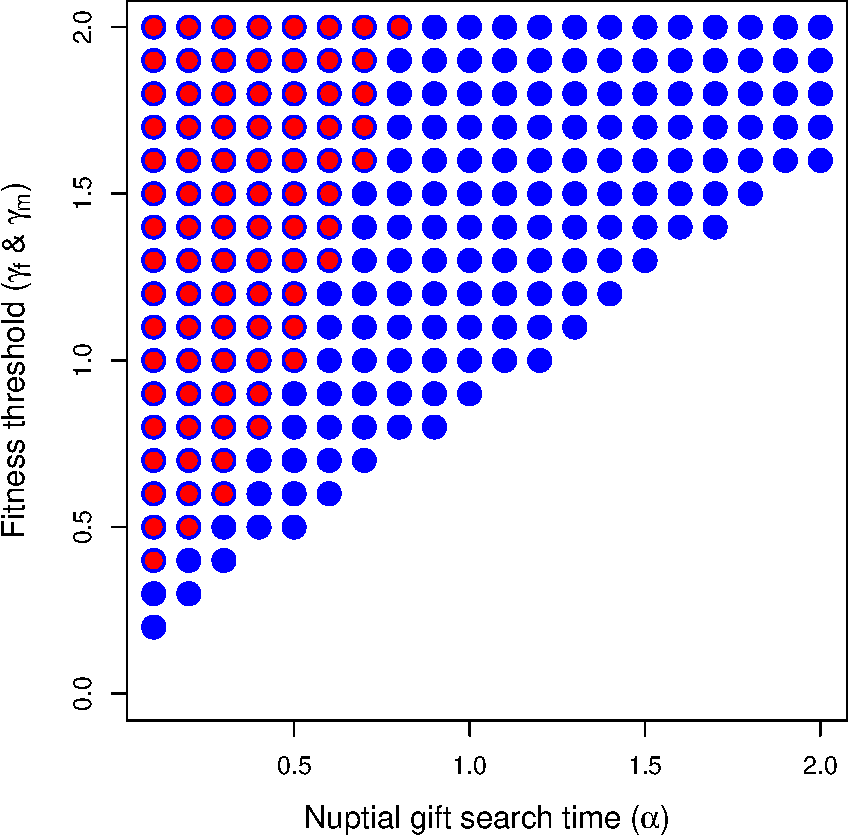
\includegraphics{SI_files/figure-latex/unnamed-chunk-9-1.pdf}
\caption{Figure S4.1: The separate evolution of male search and female
choosiness as a function of nuptial gift search time. Points show where
the lower 95\% confidence interval of male search (blue) and female
choosiness (red) exceeds zero, indicating evolution of nuptial gift
search or choosiness. Each point includes data from \(2 \times 3000\)
replicate simulations with identical starting conditions. In the first
batch, male search was constant and initialized at
\(T_{\mathrm{m}} = \alpha\), and female choice was evolving. In the
second batch, male search was evolving, and there was no option for
female choice. The parameters \(T_{\mathrm{f}}=2\), and \(\gamma\) and
\(\alpha\) values were set within the range {[}0.1, 2.0{]} and {[}0.0,
2.0{]}, respectively.}
\end{figure}

\captionsetup{labelformat=default}

\clearpage

\hypertarget{references}{%
\section*{References}\label{references}}
\addcontentsline{toc}{section}{References}

\hypertarget{refs}{}
\begin{CSLReferences}{0}{0}
\leavevmode\vadjust pre{\hypertarget{ref-Kokko2001}{}}%
Kokko, H. \& Monaghan, P. (2001)
\href{https://doi.org/10.1046/j.1461-0248.2001.00212.x}{{Predicting the
direction of sexual selection}}. \emph{Ecology Letters}, \textbf{4},
159--165.

\end{CSLReferences}

\end{document}
